% This file is the Latex source of the Big Data course project
% report. The project contributors are Ali Alavi, Rolf jagerman
% and Ken Tsay.
% The report is written by Ali Alavi.

%
\documentclass{llncs}
%

\usepackage{graphicx} % for importing images

\usepackage{subcaption} % for subfigures
\captionsetup{compatibility=false} % to make subfigures compatible with template

\usepackage{url} % for URL references
\usepackage{float} % helps with locating the 
\usepackage[T1]{fontenc}  % providing font encoding
% used for drawing the diagrams
%
\begin{document}
%
\mainmatter              % start of the contributions
\pretolerance=10000  % This avoids long lines
\pagestyle{headings}

%
\title{Automatic News Generation Based on Twitter}
%
\titlerunning{Automatic News Generation Based on Twitter}  % abbreviated title (for running head)
%                                     also used for the TOC unless
%                                     \toctitle is used
%
\author{Ali Alavi\inst{1} \and Rolf Jagerman\inst{1} \and
Tsay Kai-En\inst{1}}
%
\authorrunning{Ali Alavi, Rolf Jagerman and Tsay Kai-En} % abbreviated author list (for running head)
%
%
\institute{ETH Z\"urich, Z\"urich, Switzerland\\
\email{alavis@ethz.ch, \{rolfj, tsayk\}@student.ethz.ch}
}

\maketitle              % typeset the title of the contribution
%
\section{Introduction}
%
This report presents the current status of the project \textbf{Automatic News Generation Based on Twitter}, 
for \textbf{Big Data} course (code \textit{263-3010-00L}). This project tries to answer the following questions: 
\textit{Can we automatically generate news headlines based on public twitter posts? Can this method of news generation 
perform better than the available news agencies, in terms of speed, reliability and so on?}

We tackle this problem by taking the following steps:

\begin{enumerate}
  \item \textit{Data collection: }Gathering a large set of twitter posts and news headlines 
  \item \textit{Building a classifier: }Use the news headlines to train a classifier
  \item \textit{Labeling the tweets: }Label each tweet using the classifier we previously trained
\end{enumerate}

A big picture of the system is depicted in Figure ~\ref{fig:A big picture of the system}. In the rest of this report we will elaborate on the design and realization of the system.

\begin{figure}[H]
  \centering
  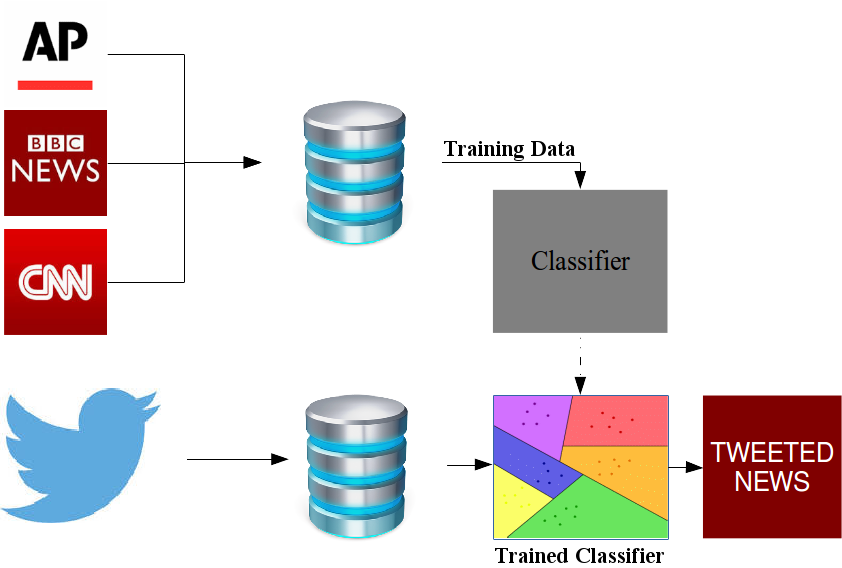
\includegraphics[width=0.8\textwidth]{images/bigpicture.png} 
  \caption{A big picture of the system}
  \label{fig:A big picture of the system}
\end{figure}

\section{Data collection}
\subsection{Data sources}
\subsubsection{Twitter data}
Twitter offer different ways of gathering data for different applications ~\cite{twitterdocumentation}. Unfortunately, giving access to the historic data is not one of them. In other words, our access to public data is limited to the most recent tweets. Hence, we decided to collect a large number of the most recent public tweets. 
Although Twitter Firehose ~\cite{twitterrestapi} offers access to all public tweets, it requires special permission to access, which we could not aquire. Luckily, Twitter's \textit{Streaming API} ~\cite{twitterstreaming} can offer a large number of tweets: it streams a random subset (around one percent) of all the public tweets. this subset is large enough for our purpose. Moreover, the streaming API allows for a much faster collection of tweets in comparison to other APIs such as \textit{REST API}, and also does not have the rate limitations imposed by Twitter on its \textit{REST} APIs ~\cite{twitterdocumentation}. 


\subsubsection{News data}
We looked into different news agencies (CNN, BBC, Reuters, USA Today, The New York Times,...) and news aggregators (Feedzilla, Google News, Bing Search, ...) in order to collect the required data for training the classifier. Unfortunately, all such sources impose some rather strict limitations on the number of requests and results an agent can send and recieve. As an example, Feedzilla has a limitation of 100 results per request. Bing news is also a commercial product costs of which we cannot afford! ~\cite{bingsearchapi}. Although we managed to collect a good amount of news using The New Your Times ~\cite{thenytimes} and USA Today ~\cite{thenytimes} APIs, we gave them up for a better news source: Twitter accounts of the news agencies. 

All news agencies that we looked for have different twitter accounts for different news categories. For the first phase of the project, we chose to use the following news categories:

\begin{enumerate}
  \item Politics
  \item Sports
  \item Technology
\end{enumerate}

These categories are chosen due to the following facts:
\begin{itemize}
  \item There is not much overlap between these news categories (cf. business, technology, finance)
  \item The frequency of the news generated in these categories are significantly higher that other categories (couple of news every hour)
\end{itemize}

We currently use the following Twitter accounts as our news sources: \textit{@CNNPolitics, @BBCPolitics, @ReutersPolitics, @BBCSport, @WorldSportCNN, @ReutersSports, @BBCTech, @CNNtech, @ReutersTech}. Each account does not have more than some thousands of Tweets, and they do not Tweet more than a couple of news per hour.

\subsection{Data storage}
To use the streaming API, the data collecting script needs to send an initial request and then keep listening for the stream of responses. Thus, we need to keep the script running on a server for a long period of time. Moreover, the API publishes more than 2000 tweets per second. This translates to around 20 gigabytes of tweets per day. This imposes a data storage problem, as our resources were rather limited at the first phase of the project. In order to address these issues, we managed to use one of the school's servers to run our script on. This server have around 200 GB of free space, which allows for almost 10 days of continous data collection. Moreover, we managed to use RAR ~\cite{wiki:RAR} compression to reduce the data size by a factor of 7. Nevertheless, since school servers are not the most reliable type of servers, we decided to take some precautions by setting up a home-based Raspberry Pi ~\cite{wiki:raspberrypi} server and connecting it to a 1-terabyte external hard disk drive (See Figure ~\ref{fig:Raspberry Pi}). Using this setup, we are capable of collecting and storing around 350 days of twitter data using the \textit{Streaming API}:
\[\textit{Days of tweet collection}=\frac{\textit{Storage size}\times \textit{Compression ratio}} {\textit{Size of tweets per day}}\]
\[\frac{\textit{1000 GB} \times 7}{\textit{20 GB per day}}=\textit{350 days} \]

\begin{figure}[H]
  \centering
  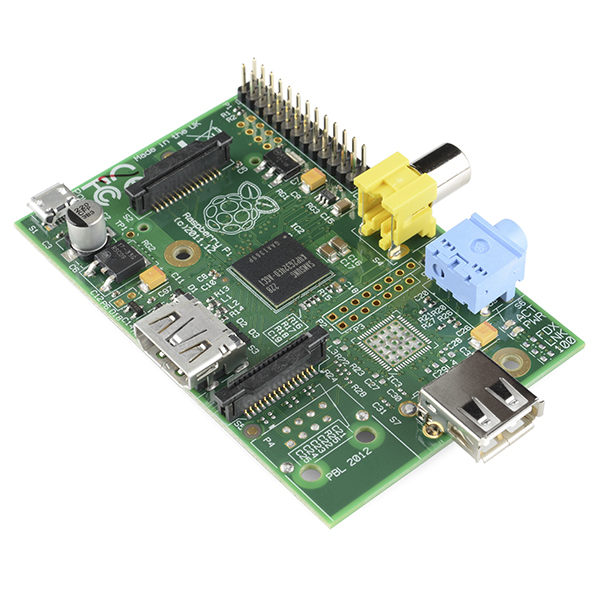
\includegraphics[width=0.5\textwidth]{images/rpi.jpg}
  \caption{Raspberry Pi Setup / Image to be updated by Ali}
  \label{fig:Raspberry Pi}
\end{figure}

\section{Classification of tweets}
To select relevant tweets from the massive amount of twitter data, we will have to classify the tweets. By accurately assigning labels to tweets that describe their topic, we can find tweets that are about interesting news topics, such as "sports", "technology" or "politics".

\subsection{Feature extraction}
Traditionally, one would have to build a dictionary of the entire corpus that is being classified before being able to turn samples into feature vectors that can be used by a classifier. This would require at least one pass over the entire data set. We wish to prevent having to iterate over the entire data set multiple times as this would be time consuming. To this end, feature hashing is used to turn text into feature vectors without requiring a dictionary. The text is tokenized, stemmed and then hashed by a fast non-cryptographic hashing algorithm into a sparse feature vector. By choosing a sufficiently large feature space we minimize the risk of collisions. The generated feature vectors can then be used by a classifier.

\subsection{Choice of classifier}
The training data, which is obtained from the news agencies, is assigned the appropriate labels and processed by a stochastic gradient descent classifier. This type of classifier can converge on a solution without having to load the entire dataset into memory. This made it a great choice for this project, as we expect the data to grow beyond the memory bounds of a standard computer.

\subsection{Labeling tweets}
After the classifier finishes training it outputs a model that can be used to label tweets. These tweets get the same preprocessing as the training data and are tokenized, stemmed and turned into feature vectors. The classifier then proceeds to predict the labels based on these feature vectors. Labeling tweets in this way is fast enough to keep up with the public sample stream of twitter on a single laptop. Furthermore, the labeling process is trivial to scale. By copying the model to different machines, and assigning different parts of the data to these machines, we can label a large amount of data.

\subsection{System overview}
A detailed diagram of the system is seen in Figure \ref{fig:System diagram}. The bottleneck of the system is the training process. The process of learning is difficult to scale.

\begin{figure}[H]
  \centering
  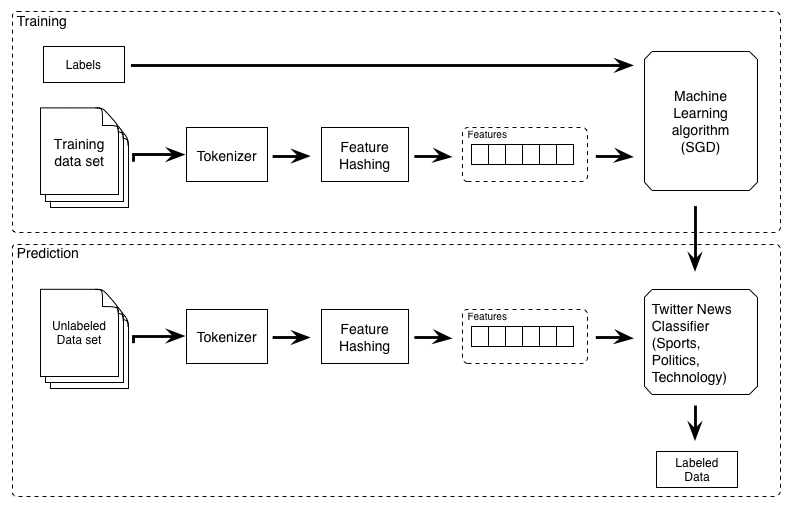
\includegraphics[width=\textwidth]{images/system.png}
  \caption{System diagram}
  \label{fig:System diagram}
\end{figure}

\section{Tools, Languages and Libraries}
Python was used as the sole programming language of the project.
In later steps we might use Java or Scala to scale the project.
We used the Python machine learning package Scikit ~\cite{scikit-learn}, which significantly simplified development of the trainer. 
[MORE HERE BY ALI, ROLF AND KEN]

\section{Results}
To measure the quality of the classifier we use several known metrics for multi-class classification. Precision, Recall and F1-Score are good indicators for the behavior of each class. Confusion matrices give quick insight in the performance of classes relative to each other.

\begin{table}
\begin{center}
\begin{tabular}{|r|r|r|r|r|} \hline
class  & precision   & recall & f1-score  & support \\ \hline
 technology    &   1.00 &     0.08  &    0.14   &   6195 \\
     sports   &    1.00   &   0.03   &   0.07   &   6365 \\
   politics   &    1.00  &    0.10   &   0.18   &   6376 \\
      other   &    0.79 &     1.00  &    0.88   &  65725 \\ \hline
avg / total  &     0.84   &   0.79  &    0.71   &  84661 \\ \hline
\end{tabular}
\end{center}
\caption{Classification performance over the three trained categories}
\label{tbl:classification-report}
\end{table}
 
\begin{figure}[H]
    \centering
    \begin{subfigure}[b]{0.48\textwidth}
        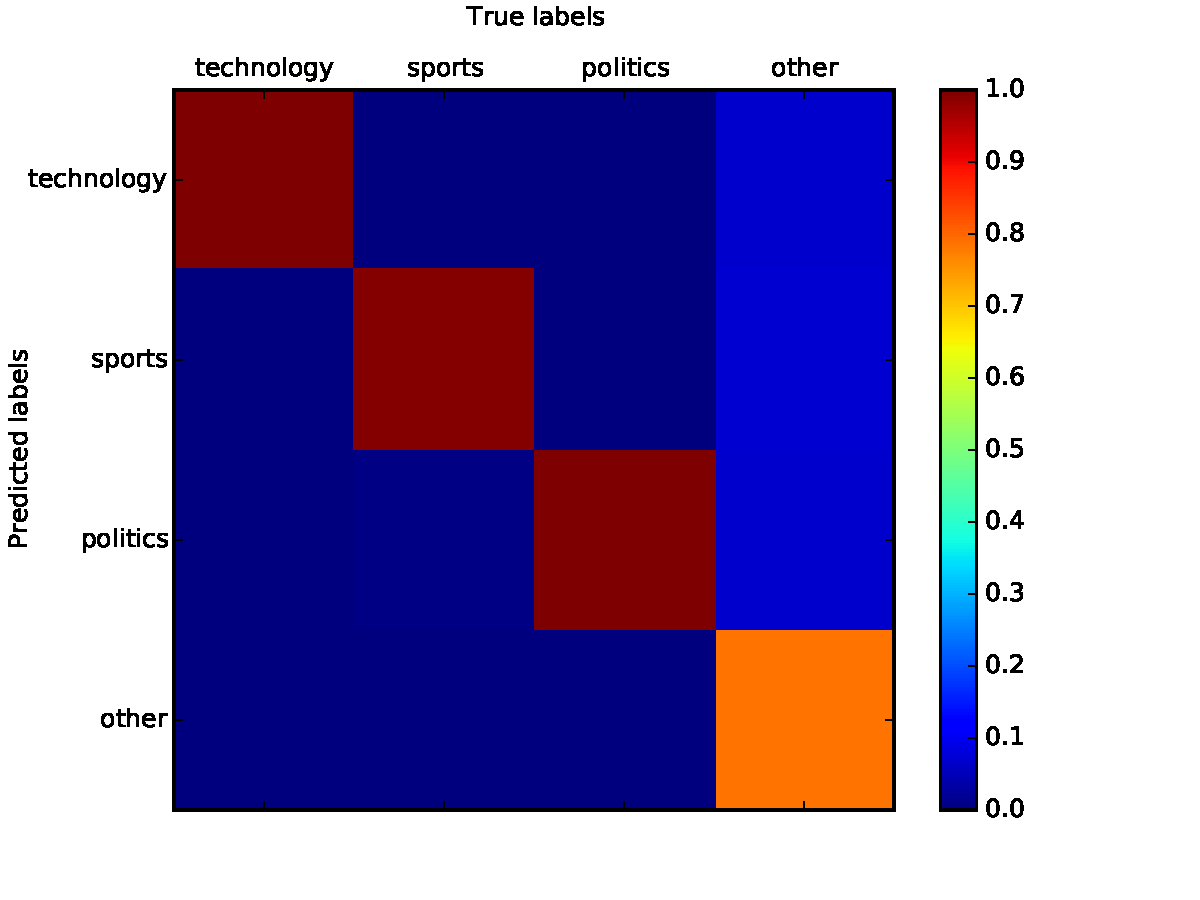
\includegraphics[width=\textwidth]{images/high-precision.pdf}
        \caption{Column-normalized confusion matrix.}
        \label{fig:column-confusion-matrix}
    \end{subfigure}
    \begin{subfigure}[b]{0.48\textwidth}
        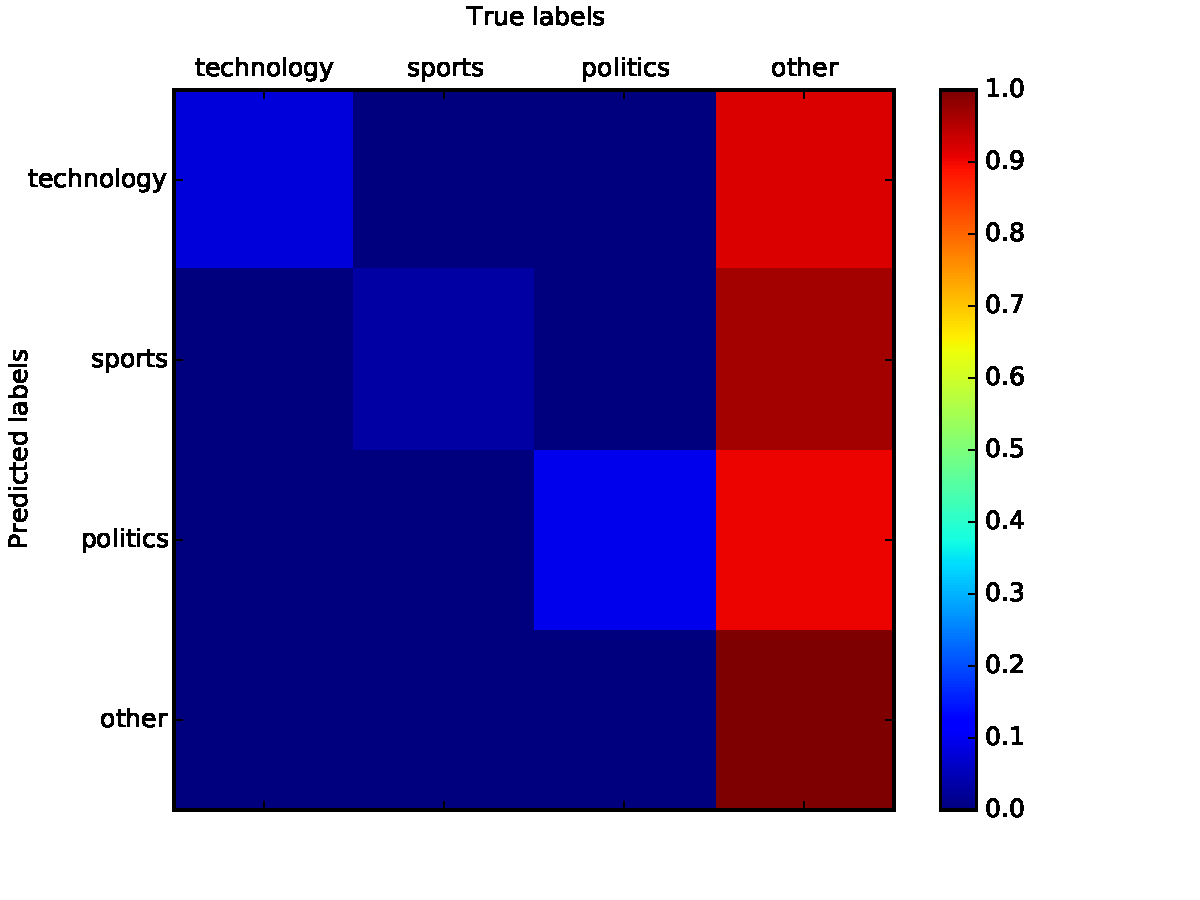
\includegraphics[width=\textwidth]{images/low-recall.pdf}
        \caption{Row-normalized confusion matrix.}
        \label{fig:row-confusion-matrix}
    \end{subfigure}
 \end{figure}

\section{Conclusion and future work}
In this report we presented the current status of a Twitter based news generator. We managed to label Tweets based on the classifier we trained using new 

\bibliographystyle{plain}
\bibliography{report.bib}

\end{document}